\chapter{Entregable 1}
\section{Transformación base de datos de la UCI (Machine learning repository) a formato .arff}

En este apartado veremos como transformar una base da datos del repositorio UCI al formato .arff.

\subsection{Base de datos Dermatology}

\begin{itemize}
\item Muchas de las bases de datos disponibles en la red se encuentran en formato .csv.
\item Además de usar ficheros .arff, Weka también permite usar ficheros .csv aunque hay que hacerlo con precaución.
\item Se pueden visualizar los ficheros con un editor de texto o mediante $ Tools \rightarrow ArffViewer $.
\end{itemize}

Una vez descargada la base de datos, la abrimos con excel. Entraremos en la opciones avanzadas en excel y cambiamos la configuración regional para que se utilice el ``.'' como separador decimal y la ``,'' como separador de miles. Una vez abierto el archivo, excel invoca el asistente de conversión de texto en el cual es importante resaltar la coma como separador de campos (Figura\ref{fig:asistente_excel}). Guardamos el fichero con formato nativo xls para tenerlos para futuras modificaciones y también lo guardamos como formato csv que si lo puede leer Weka.

\begin{figure}[H]
	\centering
    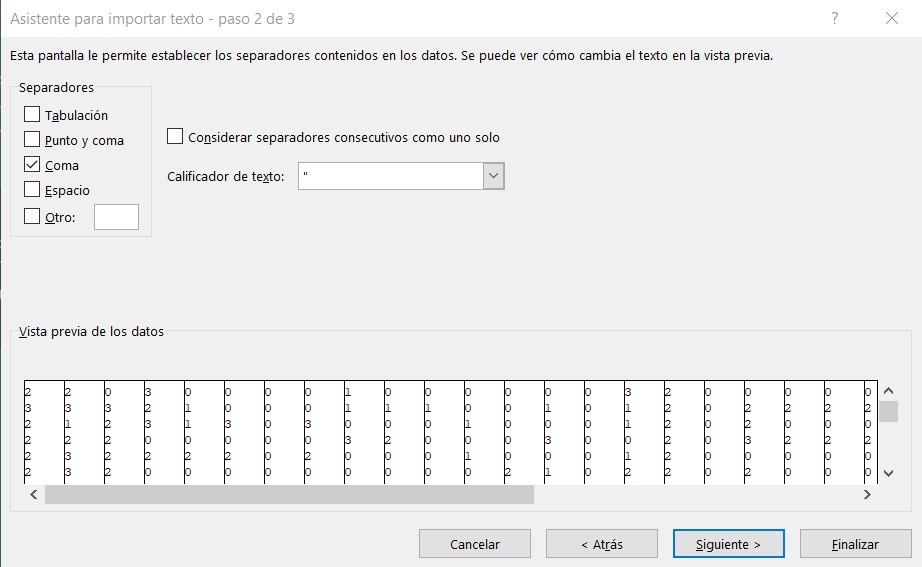
\includegraphics[width=\textwidth, height=1.05\textwidth]{asistente_conversion_excel}
    \caption{Asistente conversión Excel}
    \label{fig:asistente_excel}
\end{figure}

Abrimos weka, elegimos ``csv'' como tipo de archivo y muy importante seleccionar la opción ``invoke''. (Figura\ref{fig:invoke}).
Se nos abrirá el convertidor de Weka (Figura\ref{fig:conversor_weka}) en donde debemos cambiar algunos parámetros.
 
\begin{figure}[H]
    \centering
    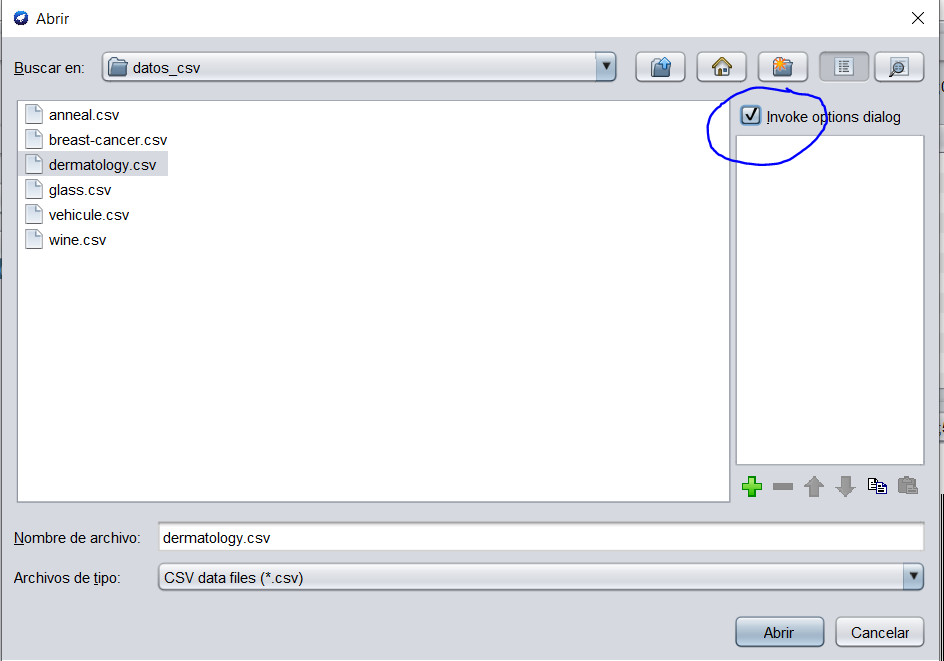
\includegraphics[width=\textwidth, height=1.15\textwidth]{weka_invoke}
    \caption{Abrir archivo en weka}
    \label{fig:invoke}
\end{figure}

\begin{figure}[H]
    \centering
    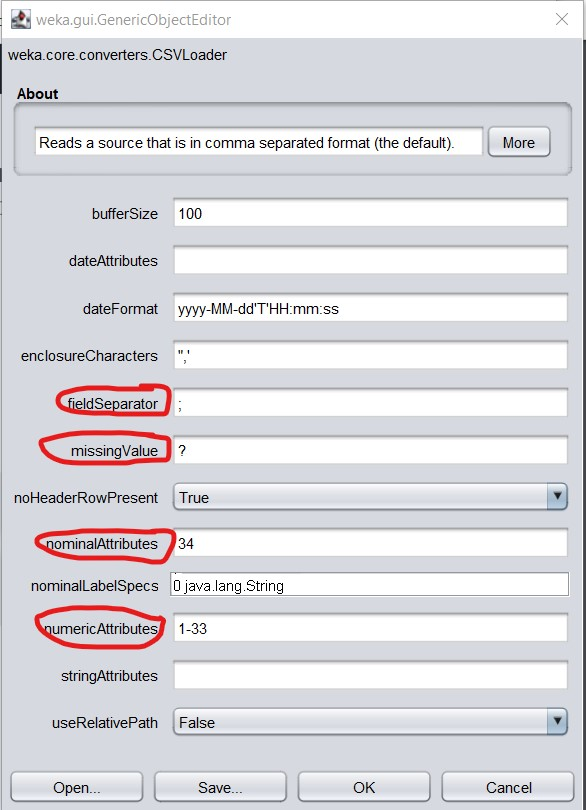
\includegraphics[width=0.7\textwidth]{Weka_convertidor}
    \caption{Convertidor Weka}
    \label{fig:conversor_weka}
\end{figure}

\begin{itemize}
\item FielSeparator: Separador de campos que será ``;''.
\item MissingValue: Carácter que usaremos para valores perdidos.
\item NoHeaderRowPresent: Decimos si el fichero no trae una fila al principio con los nombres de las variables. (En nuestro caso no la trae, decimos True).
\item NominalAttributes: Lista de variables nominales.
\item NumericAttributes: Lista de variables numéricas. (Se pueden poner rangos, ej:1-3,10-33).
\end{itemize}

Al aceptar comprobamos que nos dá un error (Figura\ref{fig:fallo}), hay problemas con la versión de Weka, por lo tanto he optado a a cambiar el fichero a mano. Para cambiar los ``;'' es mejor hacerlo con un editor de texto como Atom o Sublime Text, dandole a la tecla Control + F se abre el buscador y nos permite reemplezar todos los ``;'' por ``,'' (con esto evitamos hacerlo uno a uno) ya que Weka utiliza la coma para la separación entre los datos. En la siguiente Figura podemos ver el aspecto de los datos del fichero .arff (Figura\ref{fig:atributos}), es necesario saber de que tipo son las variables(numérica o nominal) que tenemos en la base de datos y escribirlo al principio de nuestro fichero, basta con mirar en la página UCI. (Figura\ref{fig:datos}). Por ejemplo elegimos la base de datos Dermatology (\url{https://archive.ics.uci.edu/ml/datasets/Dermatology}), pinchamos en ``Data Set Description'' y se nos descargará un fichero descriptivo sobre la base de datos, en el cual encontramos una descripción sobre la misma, número de atributos y tipo, número de instancias, clases. 

Vemos que la última columna es la clase a predecir (variable dependiente), con 5 clases distintas (1,2,3,4,5 o U). 
Los valores perdidos se representan con ``?'' y los valores no aplicables con ``-'' (y deben considerarse como categoría).

\begin{figure}[H]
    \centering
    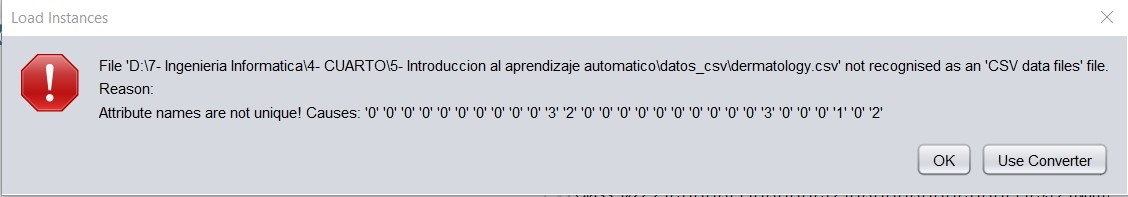
\includegraphics[width=\textwidth, height=0.35\textwidth]{error}
    \caption{Fallo del convertidor}
    \label{fig:fallo}
\end{figure}

\begin{figure}[H]
	\begin{subfigure}[H]{0.48\textwidth}
    	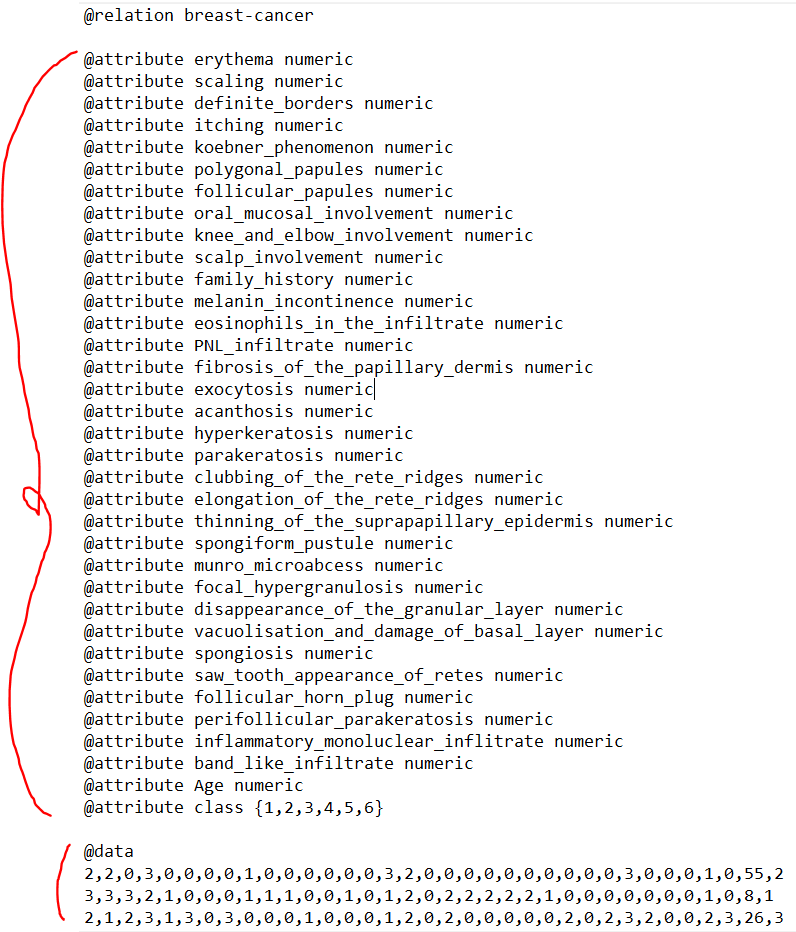
\includegraphics[width=\linewidth, height=1.5\linewidth, left]{fichero_arff}	
    	\caption{Inicio fichero}
    	\label{fig:datos}
	\end{subfigure}
	\hfill
	\begin{subfigure}[H]{0.48\textwidth}
    	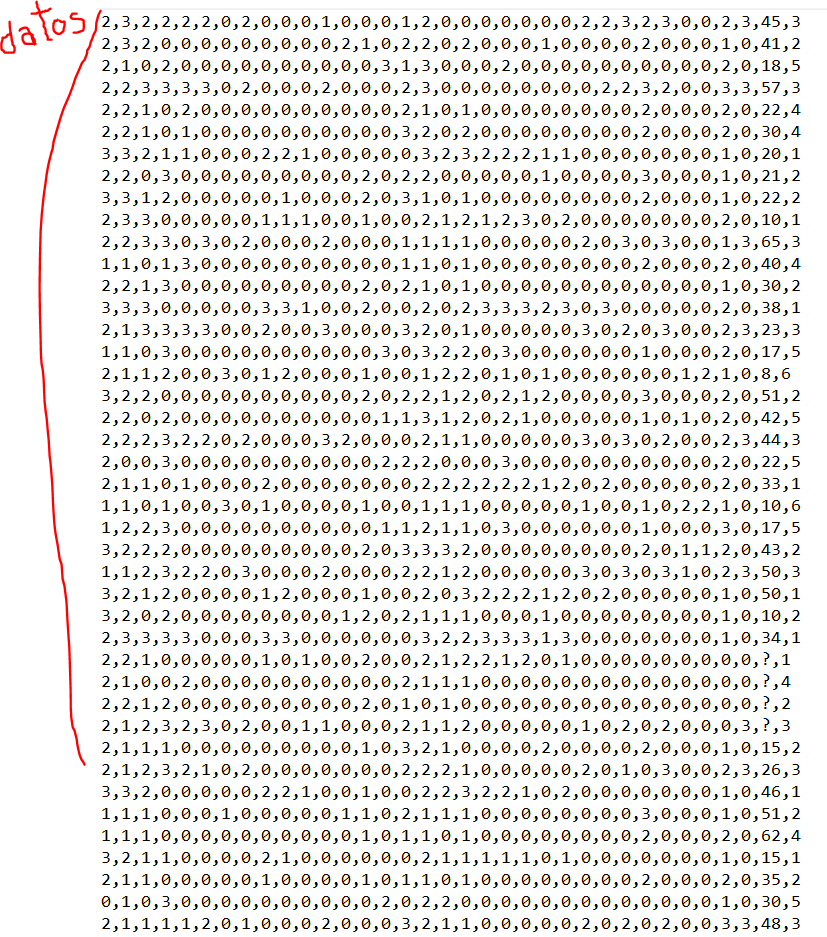
\includegraphics[width=\linewidth, height=1.5\linewidth, left]{fichero_arff2}	
    	\caption{Final fichero}
    	\label{fig:atributos}
	\end{subfigure}
	\caption{Aspecto Fichero .arff}
	\label{fig:fichero_arff}
\end{figure}

Para todas las bases de datos he realizado el mismo procedimiento:
\begin{itemize}
\item \url{https://archive.ics.uci.edu/ml/datasets/Breast+Cancer}
\item \url{https://archive.ics.uci.edu/ml/datasets/Glass+Identification}
\item \url{https://archive.ics.uci.edu/ml/datasets/Statlog+%28Vehicle+Silhouettes%29}
\item \url{https://archive.ics.uci.edu/ml/datasets/Wine}
\item \url{https://archive.ics.uci.edu/ml/datasets/Zoo}
\end{itemize}

%------------------------------------------------------------------------
%-------------------------------------------------------------------------
\newpage
\section{Filtros en Weka}

Weka permite aplicar una gran diversidad de filtros sobre los datos, permitiendo realizar transformaciones sobre ellos de todo tipo.

\begin{itemize}
	\item No tienen en cuenta el último atributo del dataset a la hora de hacer un tratamiento sobre los datos.
	\item Por defecto toman el último atributo como clase o valor numérico de salida para regresión, aplicándose el filtro a todos los patrones y atributos.
	\subitem Opción Ignore Class = false
	\item Si queremos cargar una serie de datos a los que aplicar filtros en su totalidad, indicarlo en la opción correspondiente en el filtro.
	\subitem Opción Ignore Class = true
\end{itemize}

\subsection{Base de datos audiology}
Cargue la base de datos auidiology. Pruebe todas las combinaciones posibles para pasar los atributos nominales a binarios, según los detalles proporcionados en la transparencia numero 8, mostrando en cada caso un ejemplo de cómo quedarían los nominales con 2 valores y con 3 o más valores usando esas combinaciones.
\begin{itemize}
    \item BinaryAttributesNominal=False
    \begin{figure}[H]
    \centering
    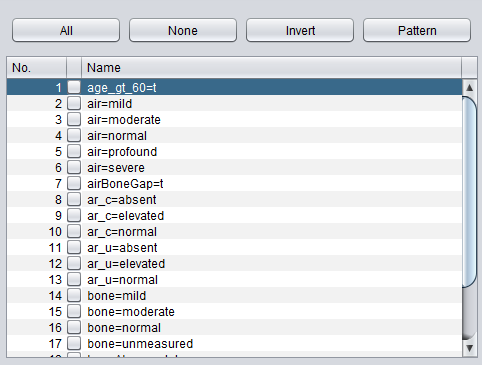
\includegraphics[width=\textwidth]{img/BAN=False.PNG}
    \caption{BinaryAttributesNominal=False}
\end{figure}

Como vemos en la figura superior, los atributos nominales con dos etiquetas como es el caso de "agegt60" se ha transformado en un solo atributo binario cuyo nombre coincide con el de una de sus etiquetas en este caso t(true) quedando con el nombre de "agegt60=t", aquellos que en este atributo posean un valor de 1 significara que tienen un valor true, para el atributo anterior, sin embargo aquellos que tengan un valor de 0 tendrían un valor de false.
Muy distinto es el caso de los atributos nominales que poseen tres o más etiquetas como es el caso del atributo air, que posee hasta cinco etiquetas, en este caso se crea un atributo para cada etiqueta indicando en cada caso con uno o cero la presencia o no de este atributo.
\end{itemize}

\begin{itemize}
    \item TransformAllValues=True
    \begin{figure}[H]
    \centering
    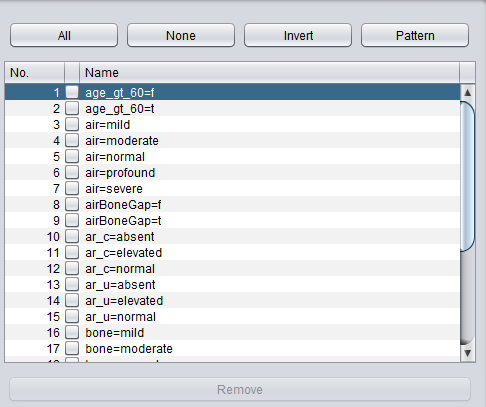
\includegraphics[width=\textwidth]{img/TAV=True.PNG}
    \caption{TransformAllValues=True}
    
\end{figure}
En este último caso vemos que tanto aquellos atributos con dos etiquetas(agegt60) que poseían las etiquetas t(true) y f(false) han sido transformados a dos atributos binarios, uno con valor de true y otro con valor de false indicando con uno o cero la presencia o no del mismo, de igual modo aquellos con tres o mas etiquetas quedan como lo hemos visto antes transformándose en tantos atributos binarios como etiquetas tuviera el atributo nominal.
\end{itemize}

\subsection{Tres filtros no supervisados}
Elija tres filtros no supervisados de los que aparecen listados, explíquelos y describa como quedan los datos antes y después al aplicarlos sobre una o varias bases de daros de las indicadas en moodle ya en formato .arff
\begin{itemize}
    \item Normalize: Normaliza todos los datos de manera que el rango de los datos pase a ser [0,1].Para normalizar un vector se utiliza la fórmula:
$$ X(i) = \dfrac{x(i)}{ \sqrt{\sum_{i=1}^{n} x(i)^2}} $$

En este caso lo vamos a aplicar a nuestra base de datos iris.arff que posee cuatro atributos numéricos y un atributo clasificador.
\begin{figure}[H]
    \centering
    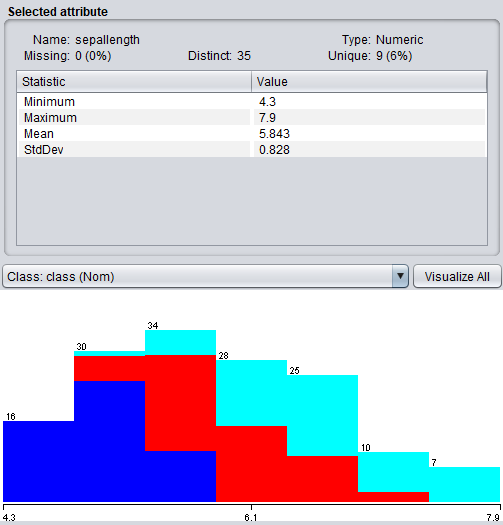
\includegraphics[width=\textwidth]{img/BN.PNG}
    \caption{Antes de aplicar filtro Normalize}
    
\end{figure}

Como vemos en la figura superior, en la cual aún no hemos aplicado el filtro Normalize, el atributo sepallenght de tipo numérico nos muestra como se encuentra repartidos los valores en función de su clase, pero siempre en un rango de entre 4,3 y 7,9. Sin embargo una vez aplicado el filtro Normalize este rango quedará normalizado entre los valores 0 y 1.
\begin{figure}[H]
    \centering
    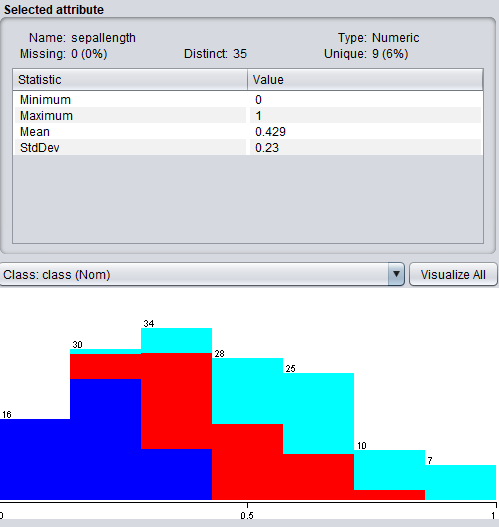
\includegraphics[width=\textwidth]{img/AN.PNG}
    \caption{Después de aplicar filtro Normalize}
\end{figure}

    \item Remove: Borra un conjunto de atributos del fichero de datos, para ello debemos de indicarle el índice de los atributos que queremos borrar de nuestro fichero de datos. A continuación se indica como hacerlo:
    \begin{figure}[H]
    \centering
    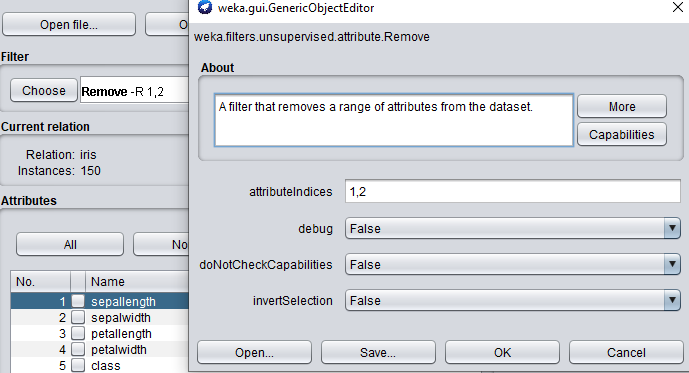
\includegraphics[width=\textwidth, height=0.7\textwidth]{img/Rem.PNG}
    \caption{Indicaciones del filtro Remove}
    \label{fig:filtro_remove}
\end{figure}

Es en el apartado ``attributeIndices'' donde indicamos los índices de los atributos que queremos borrar, podemos indicar los índices que queremos borrar o bien separados por comas o bien separados por guión lo que indicara que queremos borrar un rango de atributos.

    \item ReplaceMissingValues:
Reemplaza todos los valores indefinidos por la moda en el caso de que
sea un atributo nominal o la media aritmética si es un atributo numérico.
Para este caso hemos cogido el fichero de datos iris.arff y lo hemos modificado eliminando tres de sus valores como aparece a continuación.
 \begin{figure}[H]
    \centering
    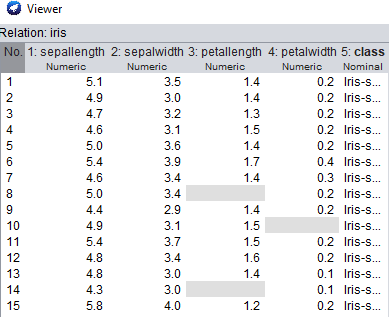
\includegraphics[width=\textwidth, height=1.1\textwidth]{img/BRP.PNG}
    \caption{Fichero con valores desconocidos}
    \label{fig:ReplaceMissingValues}
\end{figure}

En la siguiente figura se muestra como al aplicar el filtro ReplaceMissingValues los valores se han sustiudo por la media de cada atributo ya que ambos son numéricos.
 \begin{figure}[H]
    \centering
    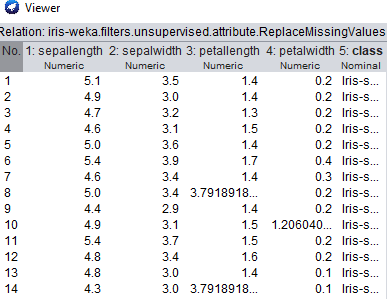
\includegraphics[width=\textwidth]{img/ARP.PNG}
    \caption{Aplicación del filtro ReplaceMissingValues}
\end{figure}

\end{itemize}

\subsection{Tres filtros supervisados}

Elija tres filtros no supervisados de los que aparecen listados, explíquelos y describa como quedan los datos antes y después al aplicarlos sobre una o varias bases de daros de las indicadas en moodle ya en formato .arff
\begin{itemize}
    \item Resample: Produce una submuestra aleatoria de un conjunto de datos utilizando muestreo con reemplazo o sin reemplazo.
El conjunto de datos original debe caber completamente en la memoria. Se puede especificar el número de instancias en el conjunto de datos generado. El conjunto de datos debe tener un atributo de clase nominal. De lo contrario, use la versión sin supervisión. El filtro se puede hacer para mantener la distribución de la clase en la submuestra o para sesgar la distribución de la clase hacia una distribución uniforme.
 \begin{figure}[H]
    \centering
    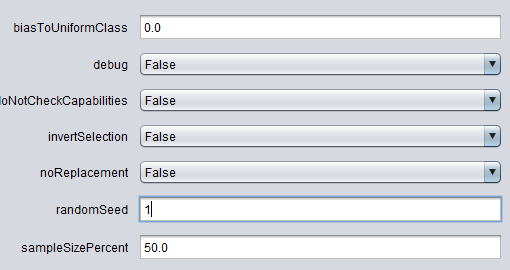
\includegraphics[width=\textwidth, height=0.8\textwidth]{img/opc_resample.PNG}
    \caption{Opciones del filtro Resample}
\end{figure}
Como vemos en la figura de arriba estas son las distintas opciones que nos plantea el filtro Resample, en este caso en particular hemos decidido el generar una nueva muestra aleatoria que siguiera la misma distribución que los datos de entrada y además tal como vemos en la ultima opción sampleSizePercent en la cual indicamos un cincuenta, esto quiere decir que el tamaño de nuestra muestra generada será del cincuenta por ciento de nuestra muestra inicial.En la siguiente figura mostramos los resultados de su aplicación.
 \begin{figure}[H]
    \centering
    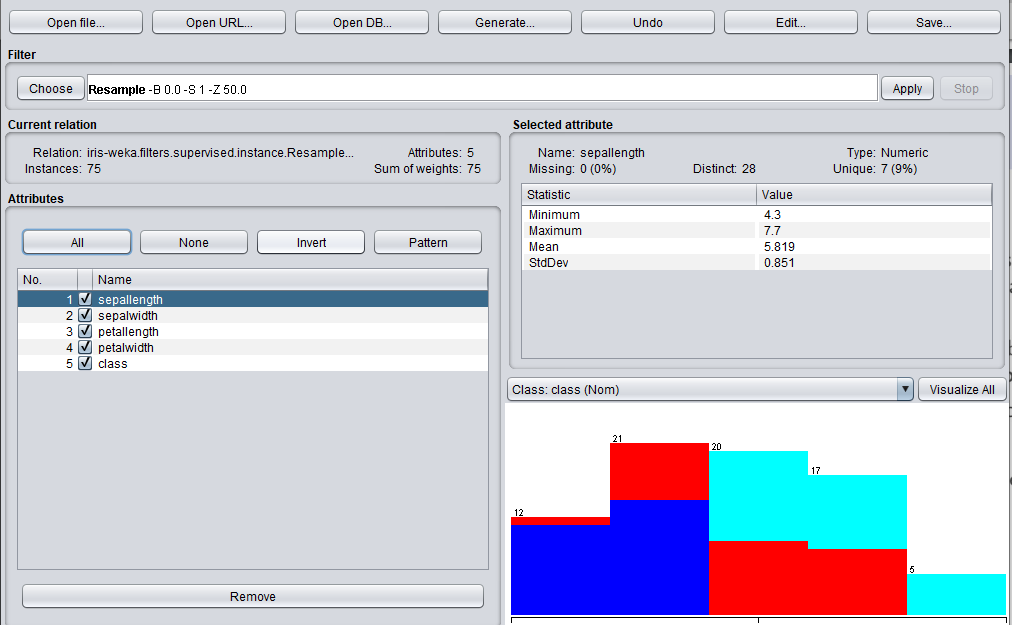
\includegraphics[width=\textwidth]{img/resample.PNG}
    \caption{Resultado de aplicar el filtro Resample}
\end{figure}
    \item SpreadSubsample: Produce una submuestra aleatoria de un conjunto de datos. El conjunto de datos original debe caber completamente en la memoria. Este filtro le permite especificar la "dispersión" máxima entre la clase más rara y la más común. Por ejemplo, puede especificar que haya como máximo una diferencia de 2: 1 en las frecuencias de clase. Cuando se usa en modo por lotes, los lotes posteriores NO se vuelven a muestrear.
    \item Discretize: Discretiza un conjunto de valores numéricos en rangos de datos. Como parámetros
    toma los índices de los atributos discretizar (attribute indices) y el número de particiones en que queremos que divida los datos (bins). Si queremos que las particiones las realice por la frecuencia de los datos y no por el tamaño de estas tenemos la opción useEqualFrecuency. Si tenemos activa esta última opción podemos variar el peso de las instancias para la definición de los intervalos con la opción DesiredWeightOfInstancesPerInterval. Si, al contrario tenemos en cuenta el número de instancias para la creación de intervalos podemos usar findNumBins que optimiza el procedimiento de confección de los mismos. Otras opciones son makeBinary que convierte los atributos en binario e invertSelection
    que invierte el rango de los atributos elegidos.
\end{itemize}



 


